%!TEX root = index.tex
\chapter[Resultados]{Resultados}
\label{chap:resultados}

Até o presente momento, os resultados deste Trabalho de Conclusão de Curso concentram-se na definição de necessidades e de parâmetros de sucesso e elaboração de possíveis soluções. 

Visto que a primeira etapa de um sistema de recomendação é a extração de informações, definimos que a aquisição de dados será feita a partir de uma base genérica, que deverá alimentar o sistema por meio de arquivos de texto com valores separados por vírgulas (\texttt{.csv}). 

A fim de facilitar o pré-processamento dos dados, exigem-se três arquivos, cada um com uma tabela de itens e seus atributos $\mathbf{A}$, clientes e suas características $\mathbf{B}$ e histórico de compras ou avaliações $\mathbf{R}$. Caso existam outras informações no banco de dados, o sistema deverá ser alterado para levar em conta o processamento dos arquivos suplementares.

\begin{equation} 
\mathbf{A} = 
\begin{bmatrix} 
 a_{i_1 f_1} &  a_{i_1 f_2} &  a_{i_1 f_3}  & \dots   \\
 a_{i_2 f_1} &  a_{i_2 f_2} &  a_{i_2 f_3}  & \dots   \\
 a_{i_3 f_1} &  a_{i_3 f_2} &  a_{i_3 f_3}  & \dots  \\ 
 \vdots &  \vdots &  \vdots  & \ddots   \\
 \end{bmatrix}
\end{equation}

\begin{equation}
	\mathbf{B} = 
\begin{bmatrix} 
 b_{u_1 c_1} &  b_{u_1 c_2} &  b_{u_1 c_3}  & \dots   \\
 b_{u_2 c_1} &  b_{u_2 c_2} &  b_{u_2 c_3}  & \dots   \\
 b_{u_3 c_1} &  b_{u_3 c_2} &  b_{u_3 c_3}  & \dots  \\ 
 \vdots &  \vdots &  \vdots  & \ddots   \\
 \end{bmatrix}
\end{equation}

\begin{equation}
	  \mathbf{R} = 
\begin{bmatrix} 
  r_{u_1 i_1} &  r_{u_1 i_2} &  r_{u_1 i_3}  & \dots   \\
 r_{u_2 i_1} &  r_{u_2 i_2} &  r_{u_2 i_3}  & \dots   \\
 r_{u_3 i_1} &  r_{u_3 i_2} &  r_{u_3 i_3}  & \dots  \\ 
 \vdots &  \vdots &  \vdots  & \ddots   \\
\end{bmatrix}
\end{equation}

Em alguns bancos de dados relacionais, a tabela de histórico também contém outras informações adicionais $\theta$, tais como método de pagamento, data da compra, data de entrega, etc., e é denominada $\mathbf{H}$.

\begin{equation} 
\mathbf{H} =
\begin{bmatrix} 
 r_{u_1 i_1} &  \theta_{h_1 1} &  \theta_{h_1 2} & \dots   \\
 r_{u_1 i_2} &  \theta_{h_2 1} &  \theta_{h_2 2} & \dots   \\
 r_{u i} &  \theta_{h 1} &  \theta_{h 2} & \dots   \\
 \vdots &  \vdots &  \vdots  & \ddots   \\
 \end{bmatrix} \\
\end{equation}

Uma vez determinada a forma de entrada de dados, definiu-se o conjunto de dados a serem utilizados. O primeiro conjunto de dados abertos é proveniente do website de recomendações de filmes MovieLens (\url{http://movielens.umn.edu}). Nessa base de dados, o catálogo de filme faz o papel de catálogo de produtos pelos quais os usuários possam se interessar, e o histórico de compras se refere à avaliação dos filmes feita por cada usuário. Outros conjuntos de dados abertos,  a serem definidos posteriormente, também poderão ser explorados pela dupla, tais como os dados de classificação de músicas do serviço Yahoo! Music (\url{http://webscope.sandbox.yahoo.com}).

Outra base que poderemos utilizar é a de dados anônimos de lojas de comércio online. Já entramos em contato com um e-commerce de vendas de passagens de ônibus interessado em sistemas de recomendação, que forneceria sua base  para nossa pesquisa. Ao longo das últimas semanas, estabelecemos os termos do contrato de confidencialidade e explicamos como seria o desenrolar do trabalho. Esperamos obter o banco de dados antes das férias escolares, a fim de aplicar os algoritmos de recomendação também nesse caso específico. Caso a parceria se concretize, será possível avaliar o desempenho do sistema de recomendação sob aspectos como aumento no número de compras, receita adicional gerada, comparação entre os métodos anteriores utilizados pela loja e o nosso sistema, etc.

Mesmo sem ter o banco de dados em mãos, já nos foi explicado sua estrutura, para que possamos adaptar a entrada e saída de dados genérica descrita acima para esse caso específico. Ele é dividido em seis diferentes tabelas. Os relacionamentos entre tabelas e seu conteúdo estão demonstrados na Figura \ref{fig:bd-clickbus}.


\begin{enumerate}
	\item Ordem (pedido)
	\item Itens da ordem
	\item Rotas
	\item Lugares
	\item Pagamentos de ordens
	\item Endereço de cobrança
\end{enumerate}

Outro tópico discutido na reunião foi a importância da data de recomendação. O sistema deve não só prever qual será a próxima viagem do usuário, mas também quanto tempo antes da viagem devemos oferecê-la ao cliente. A loja de passagens de ônibus informou que, após estudo interno, descobriu-se que 60\% das passagens são compradas até três dias antes da data de embarque. Isso mostra que uma recomendação que não leve em conta fatores como data de viagem ou sazonalidade (o número de viagens em datas comemorativas é em geral cinco vezes maior que a média diária) terá um mau desempenho.

\begin{center}
\begin{figure}[ht]
    \begin{center}
    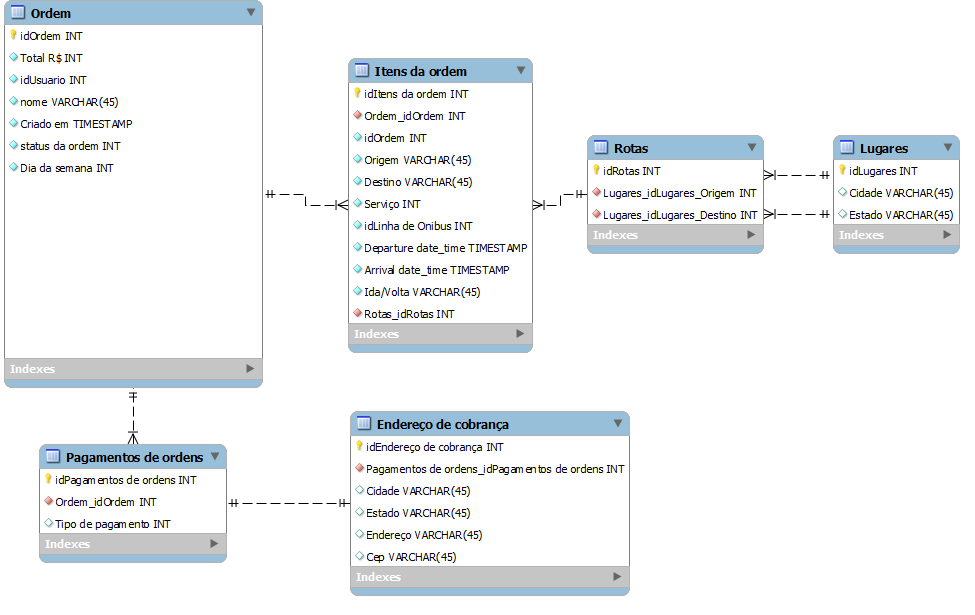
\includegraphics[width=1\textwidth]{img/estrutura-banco-de-dados}
    \end{center}
    \label{fig:bd-clickbus}
\end{figure}
\end{center}


Por fim, definimos que para qualquer que seja a aplicação, os resultados das recomendações serão entregues por meio de um arquivo \texttt{.csv}. Este conterá= o identificador de cada usuário com as recomendações de produtos, assim como o valor numérico associado à recomendação. Esse resultado é o mais importante do ponto de vista do e-commerce, que o utilizará como estratégia de marketing na sugestão de produtos.